\section{\Acl{NLP} for NMR estimation}
\label{sec:nlp}
Attention now turns to the application of \acfi{NLP} in for \ac{FID}
estimation, which in this work accepts an initial guess of parameters from
the \ac{MPM}, $\symbf{\theta}^{(0)}$, and generates the final estimate,
$\bthstar$.

\subsection{An overview of \ac{NLP}}
\label{subsec:nlp-overview}
In an optimisation problem, the goal is to determine the minimum\footnote{
    In certain applications, the interest is actually in finding the maximum of
    a function. However, it is trivial to transform a maximisation problem into
    a minimisation problem by finding the minimum of negative of the function.
}
of a function $\Fth: \mathbb{R}^n \rightarrow \mathbb{R}, n \in \mathbb{N}$, often
called the \emph{cost function} or \emph{fidelity}.
This is typically with the goal of determining the argument $\bthstar$ at
which the optimum is found:
\begin{equation}
    \bthstar = \argmin_{\bth \in \mathbb{R}^n} \Fth.
    \label{eq:minF}
\end{equation}
The above problem is \emph{unconstrained}, as there are no limitations that the
parameter vector is subjected to. Unless $\Fth$ has particular properties, such
as convexity\footnote{
    A convex function is one such that a line segment through any two points of
    the function lies above it.
}, it is generally only possible to determine a \emph{local minimum},
rather than a \emph{global minimum}. $\bthstar$ is a local
minimiser of $\Fth$ if there is a \emph{neighbourhood} $V \ni \bthstar$ for which
\begin{equation}
    \Fthstar \leq \Fth\ \forall \bth \in V.
  \label{def:local-minimiser}
\end{equation}
$V \subset \mathbb{R}^n$ is such that one can move some amount in any direction
away from $\bthstar$ and still be in $V$.

Key to \ac{NLP} are the \emph{necessary conditions}, which define whether a
given vector $\bth$ is a local minimum of$\mathcal{F}$.
The \emph{first necessary condition} states
that if $\Fth$ is continuously differentiable, and $\bthstar$ is a local extremum of
$\Fth$, then the gradient vector $\bdgthstar \coloneq \nabla \Fthstar$ is the
zero vector:
\begin{equation}
    \bdgthstar = \symbf{0} \in \mathbb{R}^n
\end{equation}
The \emph{second necessary condition} subsequently states that
if $\Fth$ and $\bdgth$ are continuously differentiable, and $\bthstar$ is a
local minimiser of $\Fth$, then the Hessian matrix $\bdHthstar \coloneq
\nabla^2 \Fthstar$ is positive semidefinite, i.e.
\begin{equation}
  \symbf{v}^{\mathrm{T}} \bdHthstar \symbf{v} \geq 0\ \forall \symbf{v} \in \mathbb{R}^n.
\end{equation}
Furthermore, it is a \emph{unique} local minimiser if the \emph{second-order
sufficient condition} is also satisfied, i.e. that the Hessian is positive
definite:
\begin{equation}
    \symbf{v}^{\mathrm{T}} \bdHthstar \symbf{v} > 0\ \forall \symbf{v} \in \mathbb{R}^n.
\end{equation}

A plethora of approaches have been established to determine local minima of
scalar functions. One of the better-known strategies is \emph{Newton's method},
in which a quadratic approximation of the fidelity is considered.
For a given iteration $k \in \mathbb{N}_0$, the fidelity is approximated using
\begin{equation}
    \FQth =
        \Fthk +
        \symbf{h}\T \bdgthk +
        \tfrac{1}{2} \symbf{h}^{\mathrm{T}} \bdHthk \symbf{h},
    \label{eq:quad-approx}
\end{equation}
where $\symbf{h} = \bth - \bthk$.  An updated prediction of the parameter
vector is derived by finding the minimum of this quadratic approximation:
\begin{gather}
    \frac{\partial \Fth}{\partial \symbf{h}} =
        \bdgthk + \bdHthk \symbf{h} \notag\\
    \implies 0 = \bdgthk + \bdHthk \left(\bthkplusone - \bthk\right) \notag\\
    \therefore\ \bthkplusone =
        \bthk - \bdHthk^{-1}
        \bdgthk.\label{eq:newton-update}
\end{gather}
This process is repeated, until the convergence criterion as been met:
\begin{equation}
    \left\lVert \bdgthk \right\rVert \leq \epsilon.
\end{equation}
The threshold $\epsilon > 0$, can be tuned based on the desired accuracy of the
result, and is usually several order of magnitude less than $1$.
\Cref{eq:newton-update} tends not to be used as the update formula in real
optimisation problems. One of the major downsides of the Newton update is the
possibility that is not a minimising update if the Hessian is not positive
definite. Two primary strategies have emerged which are typically used instead:
\begin{itemize}
    \item \emph{Line search methods}\cite[Chapter 3]{Nocedal2006} determine an
        appropriate direction $\symbf{p}^{(k)}$ along which the updated
        parameter vector is sourced.  After this, an appropriate step length
        $\alpha^{(k)}$ is determined\,---\,typically in an efficient, though not
        optimal manner; abiding by the \emph{Wolfe conditions} is a common
        approach\,---\,leading to $\bthkplusone = \bthk -
        \alpha^{(k)}\symbf{p}^{(k)}$.
    \item \emph{Trust region methods}\cite[Chapter 4]{Nocedal2006} define a
        radius $\Updelta^{(k)} > 0$, and determine the minimum of
        \cref{eq:quad-approx} subject to the constraint that
        $\left\lVert\symbf{h}\right\rVert \leq \Updelta^{(k)}$.
\end{itemize}
A trust region method is applied in this work, and as such further
consideration of it will now be made.

\subsubsection{Trust Region Methods}

\begin{algorithm}
    \caption[
        Nonlinear programming routine employed in \acs{EsPy}.
    ]
    {
        Nonlinear programming routine employed in \acs{EsPy}. This makes use of
        Algorithms 4.1 \& 7.2 in \cite{Nocedal2006}, with a extra check
        inserted to deal with any negative-amplitude oscillators which may be
        generated as the routine evolves.
    }
    \label{alg:nlp}
    \begin{algorithmic}[1]
        \Procedure {NLP}{$\bY \in \mathbb{C}^{\None \times \cdots \times \ND}, \bthzero \in \mathbb{R}^{2(D + 1)M}$}
            \State $\trustradius{0} \gets \nicefrac{1}{10} \left\lVert \bdgthzeroY \right\rVert$;
            \State $\trmax \gets 16 \trustradius{0}$;
            \For {$k = 0, 1, \cdots $}
            \State $\symbf{p}^{(k)} \gets \textsc{SteihaugToint}\left(\symbf{Y}, \symbf{\theta}^{(k)}, \trustradius{k}\right)$;
                \Comment{See \cref{alg:steihaug-toint}}
                \State $\rho^{(k)} \gets
                    \frac
                        {\Fphithk - \Fphithkpk}
                        {\FphiQthk - \FphiQthkpk}$;
                \If {$\rho_k < \nicefrac{1}{4}$}
                \label{state:decrease-tr-start}
                \State $\trustradius{k+1} \gets \nicefrac{1}{4} \trustradius{k}$;
                    \label{state:decrease-tr-end}
                    \ElsIf {$\rho_k > \nicefrac{3}{4}$ \textbf{ and } $\left\lVert \symbf{p}^{(k)} \right\rVert = \trustradius{k}$}
                \label{state:increase-tr-start}
                \State $\trustradius{k+1} \gets \min\left(2 \trustradius{k}, \trmax\right)$;
                    \label{state:increase-tr-end}
                \Else
                \State $\trustradius{k+1} \gets \trustradius{k}$;
                \EndIf
                \If{$\rho^{(k)} > \nicefrac{3}{20}$}
                \label{state:large-rho-start}
                    \State $\bthkplusone \gets \bthk + \symbf{p}^{(k)}$;
                    \label{state:large-rho-end}
                \Else
                \label{state:small-rho-start}
                    \State $\symbf{\theta}^{(k+1)} \gets \symbf{\theta}^{(k)}$;
                    \label{state:small-rho-end}
                \EndIf
                \If{$k \bmod 25 = 0 \textbf{ and } \symbf{\theta}^{(k+1)}$ contains negative amplitudes}\label{state:neg-amp-start}
                    \State $\symbf{\theta}^{(0)} \gets \symbf{\theta}^{(k+1)}$ with negative-amplitude oscillators removed;
                    \State $\symbf{\theta}^{(*)}, \symbf{\epsilon}^{(*)} \gets \operatorname{NLP}\left(\symbf{Y}, \symbf{\theta}^{(0)}\right)$;
                \EndIf\label{state:neg-amp-end}
                \If{$\left\lVert \bdgthkplusone \right\rVert < \num[print-unity-mantissa=false]{1e-8}$}
                    \State \textbf{break};
                \EndIf
            \EndFor
            \State $\symbf{\theta}^{(*)} \gets \symbf{\theta}^{(k+1)}$
            \State $\symbf{\epsilon}^{(*)} \gets
                \sqrt{
                    \frac
                    {
                        \Fthstar \diag \left(
                            \left[\bdHthstar\right]^{-1}
                        \right)
                    }
                    {(\None \cdots \ND) - 1}
                }$
            \State \textbf{return} $\symbf{\theta}^{(*)}, \symbf{\epsilon}^{(*)}$;
        \EndProcedure
    \end{algorithmic}
\end{algorithm}

The structure of a typical trust region method is presented in
\cref{alg:nlp} (ignoring \crefrange{state:neg-amp-start}{state:neg-amp-end}, which is a custom addition,
see \cref{subsec:phase-variance}). An initial radius for the trust region
$\trustradius{0}$ is defined, along with a maximum permitted radius
$\trmax$, to ensure that excessively adventurous steps do not take place.
For each iteration $k$, a solution to the following sub-problem is sought:
\begin{equation}
    \begin{split}
        \bthkplusone = \argmin_{\bp \in \mathbb{R}^{n}}
            \Fthk +
            (\bthk + \bp)\T \bdgthk +
            \tfrac{1}{2} (\bthk + \bp)\T \bdHthk (\bthk + \bp) \\
        \text{subject to } \left \lVert \bp \right \rVert \leq \trustradius{k}.
    \end{split}
\end{equation}
This sub-problem is not usually minimised exactly, but instead an efficient
means of determining a sufficiently update is used.
Common approaches include computing the Cauchy point, the Dogleg
method, and a truncated conjugate-gradient
approach commonly called the \ac{ST} method\cite[Chapter 7]{Nocedal2006}.
The latter is employed in this work (see \cref{alg:steihaug-toint} and
\cref{lst:tr}). In the \ac{ST} approach, iterates of the conjugate-gradient
method\cite[Chapter 5]{Nocedal2006} are used, until either they go beyond the
trust region, or negative curvature is discovered.

Once a provisional update $\bthkplusone \coloneq \bth + \bpk$ is determined, a
metric is considered which indicates how effectively the quadratic estimate at
the proposed update $\bthkplusone = \bthk
+ \bpk$ agrees with the true value of the fidelity at this point:
\begin{equation}
    \rho^{(k)} = \frac
        {\Fthk - \Fthkpk}
        {\FQthk - \FQthkpk}.
\end{equation}
$\rho^{(k)}$ is the ratio between the actual reduction of the fidelity caused
by taking the proposed step, and the predicted reduction based on the quadratic
model. If $\rho^{(k)}$ is sufficiently close to $1$, the quadratic model being
used to generate new iterates is deemed to be acting well enough to warrant
accepting the proposed update
(\crefrange{state:large-rho-start}{state:large-rho-end}).
Furthermore, if $\rho^{(k)}$ is particularly close to 1, and the proposed
update is at the boundary of the trust radius, it is appropriate to enlarge the
radius of the trust region for the next iteration in an attempt to increase the
rate of convergence
(\crefrange{state:increase-tr-start}{state:increase-tr-end}).
On the other hand, a small value of $\rho^{(k)}$ implies that the
quadratic model reflects the true fidelity poorly, such that the proposed
update should be rejected
(\crefrange{state:small-rho-start}{state:small-rho-end}).
As well as this, the trust region's radius should be
decreased such that the model is more likely to behave faithfully
(\crefrange{state:decrease-tr-start}{state:decrease-tr-end}). The exact
thresholds which dictate whether to accept an update, and whether to adjust the
trust region radius are customisable. The hard-coded numerical values found in
\cref{alg:nlp} are the values used for the results acquired in this work.

\subsection{Non-linear programming applied to FID estimation}
\begin{remark}
    \label{rem:norm-data}
    Prior to estimating the dataset, it is normalised, such that the signal
    actually under consideration is $\nicefrac{\bY}{\lVert \bY \rVert}$.
    To make the result reflect the actual dataset, the final amplitudes $\bdastar$
    are multiplied by $\lVert \symbf{Y} \rVert$.
\end{remark}
Focussing now on the problem of FID estimation, the fidelity $\FthY
: \mathbb{C}^{\None \times \cdots \times \ND} \times
\mathbb{R}^{2(1 + D)M} \rightarrow \mathbb{R}$ is given by
\begin{equation}
    \FthY = \left \lVert \bY - \bXth \right \rVert^2.
    \label{eq:fidelity}
\end{equation}
The elements of the gradient vector $\bdgthY \in \mathbb{R}^{2(1+D)M}$ and
the Hessian matrix $\bdHthY \in \mathbb{R}^{2(1+D)M \times 2(1+D)M}$ are then
derived by taking the first and second partial derivatives of the fidelity with
respect to the elements in $\bth$, respectively:
\begin{subequations}
    \begin{gather}
        g_i = -2 \Re
                \left\langle
                    \left(\bY - \bX\right),
                    \frac{\partial \bX}{\partial \theta_i}
                \right\rangle,
        \label{eq:grad} \\
        h_{i,j} = 2 \Re
            \biggl(
                \underbrace{
                    \left\langle
                        \frac{\partial \bX}{\partial \theta_i},
                        \frac{\partial \bX}{\partial \theta_j}
                    \right\rangle
                }_{\circled{1}}
                -
                \underbrace{
                    \left\langle
                        \left(\bY - \bX\right),
                        \frac{\partial^2 \bX}{\partial \theta_i \partial \theta_j}
                    \right\rangle
                }_{\circled{2}}
            \biggl).
            \label{eq:hess}
    \end{gather}
    \label{eq:fidelity-grad-hess}
\end{subequations}
$\forall i,j \in \lbrace 1, \cdots, 2(1+D)M \rbrace$.
The complete set of first and second derivatives of a particular element of the
model $x \coloneq \xnonenD$, given by \cref{eq:x}, is as follows
$\forall m \in \lbrace 1, \cdots, M \rbrace$,
$\forall d, d^{\prime} \in \lbrace 1, \cdots, D \rbrace$:
\begin{subequations}
    \begin{gather}
        \xderiv{\theta_m} \equiv
            \xderiv{a_m} =
            \frac{x}{a_m},\\
        \xderiv{\theta_{m + M}} \equiv
            \xderiv{\phi_m} =
            \iu x,\\
        \xderiv{\theta_{m + (d + 1)M}} \equiv
            \xderiv{\fdm} =
            2 \pi \iu \Dtd \nd x,\\
        \xderiv{\theta_{m + (d + D + 1)M}} \equiv
            \xderiv{\etadm} =
            - \Dtd \nd x,\\
        \xderivtwosame{\theta_{m}} \equiv
            \xderivtwosame{a_m} =
            0,
            \label{eq:amp-second-deriv}\\
        \xderivtwodiff{\theta_{m}}{\theta_{m + M}} \equiv
            \xderivtwodiff{a_m}{\phi_m} =
            \frac{\iu x}{a_m},\\
        \xderivtwodiff{\theta_{m}}{\theta_{m + (d + 1)M}} \equiv
            \xderivtwodiff{a_m^{\vphantom{(d)}}}{\fdm} =
            \frac{2 \pi \iu \Dtd \nd x}{a_m},\\
        \xderivtwodiff{\theta_{m}}{\theta_{m + (d + D + 1)M}} \equiv
            \xderivtwodiff{a_m^{\vphantom{(d)}}}{\etadm} =
            \frac{-\Dtd \nd x}{a_m},\\
        \xderivtwosame{\theta_{m + M}} \equiv
            \xderivtwosame{\phi_m} =
            -x,\\
        \xderivtwodiff{\theta_{m + M}}{\theta_{m + (d + 1)M}} \equiv
            \xderivtwodiff{\phi_m^{\vphantom{(d)}}}{\fdm} =
            -2 \pi \Dtd \nd x,\\
        \xderivtwodiff{\theta_{m + M}}{\theta_{m + (d + D + 1)M}} \equiv
            \xderivtwodiff{\phi_m^{\vphantom{(d)}}}{\etadm} =
            -\iu \Dtd \nd x,\\
        \xderivtwodiff{\theta_{m + (d + 1)M}}{\theta_{m + (d^{\prime} + 1)M}} \equiv
            \xderivtwodiff{\fdm}{\fdmp} =
            -4\pi^2 \left(\Dtd \nd \right) \left(\Dtdp \ndp \right) x,\\
        \xderivtwodiff{\theta_{m + (d + 1)M}}{\theta_{m + (d^{\prime} + D + 1)M}} \equiv
            \xderivtwodiff{\fdm}{\etadmp} =
            -2 \pi \iu \left(\Dtd \nd \right) \left(\Dtdp \ndp \right) x,\\
        \xderivtwodiff{\theta_{m + (d + D + 1)M}}{\theta_{m + (d^{\prime} + D + 1)M}} \equiv
            \xderivtwodiff{\etadm}{\etadmp} =
            \left(\Dtd \nd \right) \left(\Dtdp \ndp \right) x,\\
        \xderivtwodiff{\theta_{i}}{\theta_{j}} =
            \xderivtwodiff{\theta_{j}}{\theta_{i}},
            \label{eq:symmetric-second-derivs}\\
        \xderivtwodiff{\theta_{i}}{\theta_{j}} = 0\ \text{ if not specified above.}
        \label{eq:zero-second-deriv}
    \end{gather}
\end{subequations}
\Cref{eq:zero-second-deriv} indicates that any second derivative
with respect to two parameters which do not belong to the same oscillator will
always be $0$. This, along with the symmetrical nature of the second derivatives, see
\cref{eq:symmetric-second-derivs}, drastically reduces the required
number of second derivatives to compute, from $4 (1 + D)^2 M^2$ per data-point
to  $(1+D)\left(3 + 2D\right)M$. Finally, \cref{eq:amp-second-deriv}
indicates that another $M$ second derivatives do not need to be computed. See
\cref{tab:number-of-derivatives} for the total number of derivatives that need
to be computed for signals with different numbers of dimensions.
\begin{table}
    \begin{center}
        \begin{tabular}{ c c c }
            \toprule
            dimensions &
                \# 1\textsuperscript{st} derivatives &
                \# 2\textsuperscript{nd} derivatives\\
            \midrule
            $1$ & $4M\None$ & $9M\None$\\
            $2$ & $6M\None\Ntwo$ & $20M\None\Ntwo$\\
            $3$ & $8M\None\Ntwo\Nthree$ & $35M\None\Ntwo\Nthree$\\
            $D$ &  $2(1 + D)M \None \cdots \ND$ &  $((1 + D)(2(1 + D) + 1) - 1)M \None\cdots\ND$\\
            \bottomrule
        \end{tabular}
    \end{center}
    \caption{
        The number of first and second derivatives that are necessary to
        compute both the gradient vector and Hessian matrix of the fidelity for
        1- 2- and 3-dimensional datasets, as well as a general $D$-dimensional
        dataset.
    }
    \label{tab:number-of-derivatives}
\end{table}

\subsection{Approximating the Hessian}
Despite many of the model second derivatives being $0$, computation of those
that are not zero, and subsequently using these the form the Hessian matrix, is
often the most computationally expensive part of the optimisation. There are a
large number of optimisation problems where this is the case, and as such
there is considerable precedent for improving the efficiency of optimisation
algorithms by generating approximations of the Hessian which are less expensive.
Examples include the \ac{GN} method and \ac{LM} algorithm,
which are specifically for residual sum-of-squares problems\cite[Chapter
10]{Nocedal2006}, as well as quasi-Newton methods such as the BFGS
method\cite[Chapter 6]{Nocedal2006}.

The \ac{GN} and \ac{LM} approaches replace the true Hessian matrix at each
iteration with the following expression:
\begin{equation}
    h_{i,j} \approx 2 \Re
        \left\langle
            \frac{\partial \bX}{\partial \theta_i},
            \frac{\partial \bX}{\partial \theta_j}
        \right\rangle,
    \label{eq:hess-approx}
\end{equation}
i.e. term \circled{2} in \cref{eq:hess} involving the second derivatives is
neglected. All that needs to be generated is the Jacobian
$\symbf{J} = \nicefrac{\partial \bX}{\partial \bth}$. This often
brings a very large reduction in the computational cost, as no extra
derivatives need to be computed for the Hessian at all, since the Jacobian is
already required for generating the gradient vector.
In situations where the residuals between the data and model are small, term
\circled{1} will tend to dominate term \circled{2}, and as such these methods
often enjoy a convergence rate close to that of Newton's method when close to
local minima. Despite this, by invoking this approximation, the rate of
convergence, i.e. the number of iterations required to reach $\bthstar$, tends
to be adversely affected. See \cref{subsec:optim-vis} for an example of
this phenomenon.

\subsection{Estimation Errors}
\label{subsec:errors}
The vector of standard errors associated with the \ac{NLP} routine is related
to the \emph{observed Fisher information matrix} at convergence\cite[Section
2.7]{Pawitan2001}:
\begin{equation}
    \symbf{\epsilon}\left(\bthstar\right) = \sqrt{\diag\left(\symbf{I}\left( \bthstar \right)^{-1}\right)},
\end{equation}
where the observed Fisher Information matrix contains the negative partial second
derivatives of the log-likelihood with respect to $\bth$:
\begin{equation}
    \symbf{I}\left(\bth\right)_{i, j} =
        -\frac
        {\partial^2 \ell \left( \bdthY \right)}
        {\partial \theta_i \partial \theta_j}.
\end{equation}
Recalling the form of the log-likelihood given by \cref{eq:log-likeihood},
the elements of $\symbf{I}\left(\bth\right)$ are
\begin{equation}
    \symbf{I}\left(\bth\right)_{i, j} =
        -\frac{1}{\sigma^2}
        \Re
        \biggl(
            \left\langle
                \frac{\partial \bX}{\partial \theta_i},
                \frac{\partial \bX}{\partial \theta_j}
            \right\rangle
            -
            \left\langle
                \left(\bY - \bX\right),
                \frac{\partial^2 \bX}{\partial \theta_i \partial \theta_j}
            \right\rangle
        \biggl),
\end{equation}
which very closely resembles the Hessian of $\bth$:
\begin{equation}
    \symbf{I}\left(\bth\right)_{i,j} =
        \frac{1}{2 \sigma^2} \left(
            \bdHth_{i,j}
        \right).
\end{equation}
The standard errors therefore take the form
\begin{equation}
    \symbf{\epsilon}\left(\bthstar\right) =
        \sqrt{
            2\sigma^2 \diag \left(
                \bdHthstar^{-1}
            \right)
        }.
\end{equation}
Considering that the mean and variance of the noise $\bW$ are $0$ and $2\sigma^2$, respectively:
\begin{equation}
    2 \sigma^2 = \frac{1}{\mathfrak{N} - 1}
    \left\lVert \bW \right\rVert^2 =
    \frac{1}{\mathfrak{N} - 1} \left \lVert
        \bY - \bXthstar
    \right \rVert^2,
\end{equation}
so that finally a useable expression for the standard errors is arrived at:
\begin{equation}
    \symbf{\epsilon}\left(\bthstar\right) =
        \sqrt{
            \frac
            {
                \Fthstar \diag \left(
                    \left[\bdHthstar\right]^{-1}
                \right)
            }
            {\mathfrak{N} - 1}
        }
\end{equation}

\subsection{Visualisation of a simple example}
\label{subsec:optim-vis}
\begin{figure}
    \centering
    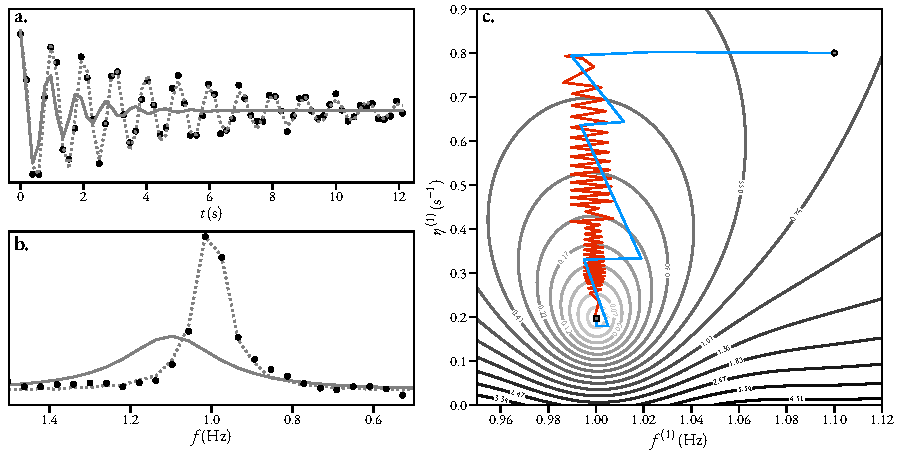
\includegraphics{optimisation_visualisation/optimisation_visualisation.pdf}
    \caption[
        A visualisation of the trajectory of a 2-parameter optimisation
        involving a simulated \acs{FID} comprising a single resonance.
    ]
    {
        A visualisation of the trajectory of a 2-parameter optimisation
        involving a simulated \acs{FID} comprising a single resonance.
        \textbf{a.} \& \textbf{b.} Representations of the signal in
        the time domain and Fourier domain, respectively.
        Black dots: the signal to be estimated $\bY$.
        Solid grey line: the model generated
        using the initial guess $\bX \left( \bthzero \right)$.
        Dotted grey line: the model generated using the optimised result, $\bX
        \left( \bthstar \right)$.
        \textbf{c.} A contour plot of the fidelity.
        Blue line: the trajectory of the parameter vector with the true
        Hessian matrix used in computing each update.
        Red line: the analogous trajectory using the Hessian approximation
        in place of the true Hessian.
    }
    \label{fig:optim-vis}
\end{figure}
\Cref{fig:optim-vis} provides a visualisation of numerical optimisation
applied on a simulated \ac{FID} comprising a single resonance.
The FID was constructed using \cref{eq:general-fid} with $D=1$, $M=1$,
$\None = 64$, $\fswone = \qty{5.2}{\hertz}$ ($\Dtone \approx
\qty{0.192}{\per\second}$), and $\foffone = \qty{0}{\hertz}$.
The resonance was parameterised by $\bth \in \mathbb{R}^4$ comprising $a=1$,
$\phi=\qty{0}{\radian}$, $\fone=\qty{1}{\hertz}$, $\etaone=\qty{0.2}{\per\second}$.
White Gaussian noise was added to the FID to give it \iac{SNR} of approximately
\qty{10}{\deci\bel}. As the visualisation of 5D space is beyond the scope of
this work, only two parameters, the frequency and damping factor were optimised
from an initial guess, with the amplitude and phase being fixed to their true
values. The initial guess comprised a frequency of \qty{1.1}{\hertz}, and a
damping factor of \qty{0.8}{\per\second}, with the solid grey lines in panels a
\& b denoting the model generated using the initial guess in the time- and
Fourier-domains, respectively. $\bthzero$ was subjected to \ac{NLP} twice. In
the first instance, the exact Hessian matrix, given by \cref{eq:hess} was used
in order to compute each update step, while in the second the Hessian
approximation given by \cref{eq:hess-approx} was used. The initial
radius of the trust region was set to $\nicefrac{1}{10}$ of the gradient norm
($\approx 0.3$), which has a precedent in the literature\cite{Gould2005}. The
trajectories of the parameter vector are denoted as coloured lines in panel c.
In both cases, the \ac{NLP} routine successfully generated a result $\bthstar$
in agreement with the true frequency and damping factor used to construct the
\ac{FID}. However, it is clear that using the true Hessian matrix (blue)
led to a far better rate of convergence compared with the
approximated analogue (red), which exhibited ``zig-zagging''. This phenomenon
is often seen in gradient descent methods, in which each update occurs in the
opposite direction to the gradient.
14 iterations were required to reach the
convergence criterion $\epsilon \leq \num[print-unity-mantissa=false]{1e-8}$
when the true Hessian was used, while 81 were required for the approximated
case. While an anecdotal example, this highlights that use of the true
Hessian matrix tends to allow a better rate of convergence. However, for
\acp{FID} comprising many signals and far more points, the approximated form
often requires a shorter time to converge overall, as the cost of computing the
second derivatives required for the true Hessian dominates.

\subsection{Phase Variance Minimisation}
\label{subsec:phase-variance}
\note{Re-write this section}
While numerical optimisation procedures can return estimates $\bthstar$ which
can achieve highly accurate reconstructions of the original \acs{FID} (i.e.
$\bY$ and  $\bXthstar$ are in close agreement), the estimate won't
necessarily provide a faithful description of the physical phenomenon that has
given rise to the data. For the purposes of \ac{FID} estimation, the goal is to
ensure that each signal contributing to the \ac{FID} is described by a
single oscillator in the model. In scenarios where the model order $M$ used is
greater than the true number of resonances, over-fitting of the data will
occur, leading to spurious features in the estimation result, such as single
resonances being fit by multiple oscillators and/or noise components being fit.
To overcome this problem, it is desirable to include known information about
the signal into the optimisation routine as a means of guiding the parameter
vector to a more appropriate final value. One particular means of achieving
this which has been to found to be effective is the incorporation of the
variance of oscillator phases into the fidelity, such that it becomes
\begin{equation}
    \FphithY = \left \lVert \bY - \bXth \right \rVert^2 + \circvar,
    \label{eq:fidelity-phasevar}
\end{equation}
where $\circvar$ is the \emph{circular variance} of the oscillator phases
(\textit{vide infra}).
\begin{remark}
    The inclusion of the phase variance into the fidelity is one of the
    motivating reasons for normalising the data prior to estimation (see
    \cref{rem:norm-data}). $\circvar$ is constrained to the interval $[0, 1]$.
    If the data were not normalised, it is likely that $\lVert \bY - \bX
    \rVert^2$ would dominate $\circvar$ in \cref{eq:fidelity-phasevar},
    such that the influence of the phase variance would be negligible.
\end{remark}
For the phase variance to act effectively, it is necessary to apply
phase-correction to the data prior to estimation, as the assumption that the
phases of all contributing resonances are equal is typically
valid.
\note{Mention phase-variation of multiplet peaks in experiments where
J-coupling evolves prior to acquisition? $T_2$ for example.}
The inclusion of phase variance has also been found to be effective at purging
excessive oscillators that may be present in the initial guess $\bthzero$,
which be thought of in the following way:
\begin{enumerate}
    \item Assume that the initial guess contains more oscillators than the
        true number of resonances. In this circumstance, it is common to find
        that true resonances are fit with an acceptable oscillator, whilst
        extra oscillators exist with spurious phases on account of
        over-fitting.
    \item Unconstrained numerical optimisation is now run, with the fidelity
        given by \cref{eq:fidelity-phasevar}. The phase variance will
        force oscillators with phases that are significantly different to the
        majority of oscillators to drastically alter their phases to match
        them. For some/all of these oscillators, it may be the case that the
        optimiser drives these to acquire a negative amplitude, such that they
        act as if they have a phase of $\pi$ while ensuring that $\circvar$ is
        small.
    \item This provides a criterion for detecting oscillators which are likely
        to be excessive. Such oscillators can be purged from $\bth$ by
        periodically checking whether any amplitudes (i.e. $\bth[:M]$) have
        become negative, purging these, and re-starting the optimisation.
    \item The numerical optimisation routine is re-started each time
        oscillators are purged. Termination is achieved once the routine
        converges and no negative-amplitude oscillators exist in $\bth$.
\end{enumerate}

\subsubsection{Circular Variance}
Oscillator phases are an example of a \emph{circular variable}, in that all
phases are wrapped within an interval of width $2 \pi$. Given an unconstrained
(unwrapped) phase $\widetilde{\phi} \in \mathbb{R}$, the corresponding wrapped
phase $\phi \in \left( -\pi, \pi \right]$ is given by
\begin{equation}
    \phi = \left(\left(\widetilde{\phi} + \pi\right) \bmod 2 \pi\right) - \pi.
    \label{eq:phase_wrap}
\end{equation}
This makes the conventional (linear)
definition of variance, given by
\begin{subequations}
    \begin{gather}
        \Var_{\shortmid}\hspace*{-3pt}\left(\symbf{\phi}\right) =
            \frac{1}{M} \sum_{m=1}^{M} \left(\phi_m - \mu\left(\symbf{\phi}\right)\right)^2, \\
        \mu\left(\symbf{\phi}\right) = \frac{1}{M} \sum_{m} \phi_m,
    \end{gather}
\end{subequations}
unsuitable for phases. Consider as a simple example a scenario
where there are two oscillators with phases $\widetilde{\bdphi} = \left[ \pi +
\delta\:\:\pi - \delta \right]\T$ for some small $\delta$.
The phase variance is expected to be small as these two phases are similar.
However, with the inclusion of wrapping through application of
\cref{eq:phase_wrap}, these phases would actually be set to $\bdphi = \left[
    -\pi
+ \delta\:\:\pi - \delta \right]\T$, and the conventional definition of phase
variance would be large. It is therefore apparent that a definition of variance
which accounts for the periodicity of the phases is needed. The \emph{circular
variance} is given by\cite[Chapter 3]{Fisher1993}
\begin{subequations}
    \begin{gather}
        [0, 1] \ni \circvar = 1 - \frac{R}{M},\\
        R = \sqrt{c_{\Sigma}^2 + s_{\Sigma}^2}, \\
        c_{\Sigma} = \sum_{m} \cos \phi_m, \\
        s_{\Sigma} = \sum_{m} \sin \phi_m.
    \end{gather}
\end{subequations}
$R$ is the length of the resultant vector produced by summing $M$ unit vectors
with the angles given by $\bdphi$. In the case that all the vectors have the
same angle, $R=M$, leading to the variance being $0$ as expected. At the other
extreme, with $M$ vectors uniformly separated about the unit circle (with an
angle $\nicefrac{2 \pi}{M - 1}$ between all pairs of adjacent vectors), the
vectors will perfectly cancel, leading to $R=0$. In this case, the maximum
variance of $1$ is obtained.

The first and second derivatives of the circular variance are required for
the computation of the gradient vector and Hessian matrix. These are given by
\begin{subequations}
    \begin{gather}
        \frac{\partial \circvar}{\partial \theta_i} =
        \begin{cases}
            \frac{1}{RM}
            \left(
                c_{\Sigma} \sin \phi_{i-M} -
                s_{\Sigma} \cos \phi_{i-M}
            \right) & M \leq i < 2M\\
            0 & \text{otherwise}
        \end{cases}\\
        \frac{\partial^2 \circvar}{\partial \theta_i \partial \theta_j} =
        \begin{cases}
            \begin{split}
                \tfrac{1}{RM}\left[
                    \tfrac{1}{R^2}
                    \left(c_{\Sigma} \sin \phi_{i-M}  - s_{\Sigma} \cos \phi_{i-M} \right)^2 \right. \\
                    \left. + c_{\Sigma} \cos \phi_{i-M} + s_{\Sigma} \sin \phi_{i-M}
                    - 1
                \vphantom{\tfrac{1}{RM}}\right]
            \end{split}
            & M \leq i, j < 2M, i = j\\
            \begin{split}
                \tfrac{1}{RM}\left[
                    \tfrac{1}{R^2}
                    \left(c_{\Sigma} \sin \phi_{i-M} - s_{\Sigma} \cos \phi_{i-M} \right) \right.\\
                    \times \left(c_{\Sigma} \sin \phi_{j-M} - s_{\Sigma} \cos \phi_{j-M} \right) \\
                    \left. - \cos\left( \phi_{i-M} - \phi_{j-M} \right)
                    \vphantom{\tfrac{1}{R^2}}
                \right]
            \end{split}
            & M \leq i, j < 2M, i \neq j\\
            0 & \text{otherwise}
        \end{cases}
    \end{gather}
\end{subequations}


